\section{Estat de l'art sobre les tecnologies utilitzades}
{
    L'interès en les transmissions en directe ha fet que molts esforços d'empreses i grups de recerca
    es focalitzin en desenvolupar noves tecnologies per fer front a la creixent demanda en termes de qualitat
    i al mateix temps que donar servei cada cop a més clients. Les tecnologies que permeten aquestes transmissions
    se centren principalment en dos grups: protocols i codificacions. Això no obstant, en el nostre cas només ens centrarem
    en els protocols, perquè aquests poden funcionar independentment de les codificacions.
    
    Per tal d'entendre millor el projecte, en els següents apartats s'explicaran els principis i objectius de les
    tecnologies implicades. A l'annex 1 hi ha un resum extens de l'evolució de les tecnologies implicades fins a arribar
    la creació de QUIC o l'ús que es fa avui en dia de multicast. Es recomana donar una ullada si hi ha alguna sigla o tecnologia
    que no s'entén.
}


\subsection{Multicast}
{
    \ac{IP} va néixer com un protocol per interconnectar xarxes d'àrea local amb tecnologies diferents. Aquestes xarxes funcionaven de manera
    \textit{unicast}, un a un, o \textit{broadcast}, un per a tots. Malgrat això, l'any 1988 es va publicar el RFC 988 anomenat \cite{Host Extension for IP
    Multicasting}. Aquest proposava fer una extensió de la tecnologia IP per permetre la connexió d'un emissor a molts receptors, però no tots, només els
    que volguessin rebre la informació d'aquest.
    
    Per fer una analogia de multicast amb el nostre entorn quotidià, es podria dir que funciona com la \ac{TDT} o la ràdio. Es pot pensar com una antena que
    emet el senyal i si vols rebre el senyal únicament ficat el canal o la freqüència a la qual aquesta emet per poder rebre i veure o escoltar la
    transmissió, però si algú no la vol rebre no la pot ignorar.

    \begin{figure}[H]
        \label{fig:unicast_vs_broadcast_vs_multicast}
        \centering
        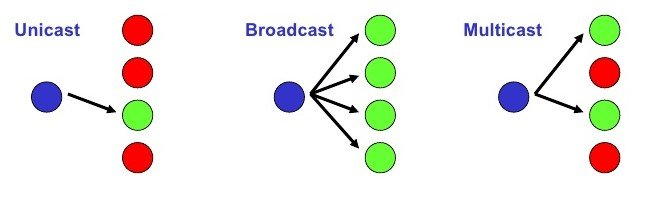
\includegraphics[width=\textwidth]{img/02_stateofart/unicast_vs_broadcast_vs_multicast.jpg}
        \caption[Unicast vs Broadcast vs Multicast]{\footnotesize{En blau l'emissor de la senyal, en verd els usuaris que reben la senyal
        i en vermell els que no. Imatge de \url{pc-solucion.es}}}
    \end{figure}

    Dins la tecnologia IP hi ha un rang d'adreces destinades a aquesta tecnologia. El rang és la classe D que va des de \textbf{224.0.0.0} fins
    \textbf{239.255.255.255}.
    
    Encara que a priori sembla una idea força senzilla, en realitat, és molt complicada, ja que té diversos problemes associats, encara que la majoria
    actualment ja tenen solució excepte un que s'esmentarà al final i és el seu gran problema a l'hora d'implementar-lo extensament. Normalment,
    les qüestions d'IP multicast se solen derivar a capes superiors.
}

\subsubsection{Multicast: IGMP}
{
    Per poder dir a un router que pot arribar a rebre l'emissió que es vol rebre aquesta es fa ús d'un protocol anomenat \ac{IGMP} o Internet Group
    Management Protocol. La idea d'aquest protocol és implementar un model de subscripció al senyal en el qual mitjançant un paquet que s'envia al
    router a una distància 1 s'informa que es vol rebre l'emissió d'una direcció destinatària i un port concrets. Aquest protocol permet també dir
    que la connexió ha d'arribar d'un lloc concret (\textit{source specific}).
}

\subsubsection{Multicast: la seguretat}
{
    Un dels majors problemes encara no resolts de multicast és l'encriptació de les comunicacions. El mètode actual per xifrar les comunicacions es
    basa a canviar la clau d'accés cada poc temps transferint-la via un canal alternatiu (via \textit{unicast}). Malgrat que aquesta solució a priori
    sembla suficient, si aquesta clau es comparteix a un usuari que no ha de poder veure el senyal (televisió de pagament per exemple) llavors la
    transmissió multicast no és segura. És més, que es comparteixi la clau per qualsevol agent escoltant el senyal pot implicar altres riscos de
    seguretat per la transmissió com la suplantació d'identitat per introduir codi maliciós.
}

\subsection{Contexte de QUIC}
{
    Transmission Control Protocol (TCP) és un protocol dissenyat per enviar un flux de dades entre dos punts. Les dades són trameses
    pel sistema TCP que s'encarrega d'assegurar que les dades arribaran a l'altre extrem exactament iguals o que en el cas que no
    fos així indicar que hi ha un error a la connexió.
    
    Per aconseguir això, TCP parteix les dades en petits paquets i afegeix una sèrie de capçaleres. Aquestes dades extres inclouen un
    número de seqüència que s'utilitza per detectar quan un paquet s'ha perdut o arribar tard (Out-of-order) i una suma de comprovació
    s'utilitza per detectar que hi ha hagut un error a les dades. Quan algun problema ocorre, TCP automàticament usa un algorisme
    que es diu Automatic Repeat Request (ARQ) en el que es notifica a l'emissor que reenvii el paquet perdut o mal transmès.
    
    En la majoria d'implementacions, quan hi ha TCP detecta un error pararà la transmissió fins que l'error s'hagi resolt o consideri
    que la connexió ha fallat. En cas de fer servir una connexió multiplexada en diversos fluxos de dades, com en el cas de HTTP/2, tots
    es veuran afectats i es pararan encara que només hi hagi hagut un error en un flux. Per exemple, si hi ha un error carregant una
    imatge d'una pàgina web, tota la resta de fluxos hauran d'esperar fins que la qüestió s'hagi solucionat. Això es coneix com la 
    qüestió d'encapçalament de línia o head-of-line blocking.
    
    TCP està dissenyat com una canonada de dades en la qual no entén el que s'està enviant. Si es requereixen necessitats addicionals
    com encriptació (TLS), aquests s'han de fer des de capes superiors a TCP, utilitzant TCP per comunicar-se amb l'altre extrem
    que utilitza software semblant. Cadascun d'aquests protocols necessita el seu propi \textit{handshake}. Normalment, això implica
    que hi hagi diversos intercanvis de paquets de sol·licitud i resposta per establir la connexió fins que aquesta finalment s'ha
    establert. Això pot arribar a ser un molt greu problema en sistemes de comunicacions amb alta latència, ja que pot significar
    sobrecàrrega de dades de control en el transcurs de la connexió.
}

\subsection{QUIC}
{   
    QUIC és un nou protocol d'Internet que es diu que canviarà com funciona actualment Internet. Daniel Stenberg, creador de
    l'aplicació curl i un dels contribuïdors a l'estàndard de QUIC, va dir que fins ara HTTP s'ha fet sobre TCP i això ha
    implicat grans limitacions, però amb la vinguda d'aquest nou protocol (QUIC), les regles del joc podran canviar
    millorant les velocitats i altres aspectes de l'Internet actual.

    A principis de la dècada passada, a Google varen començar a platejar un nou estàndard pensat per substituir TCP i al mateix
    temps simplificar i millorar coses com la seguretat o que l'establiment del canal fos el més ràpid possible inclús arribant
    al punt que en la primera resposta el servidor pogués donar informació útil al client. Amb aquesta idea en ment varen
    començar a treballar en el que anomenaren Quick UDP Internet Protocol o QUIC.

    Avui en dia es tracta d'un estàndard redactat publicat en els RFC 8999 (Version-independent Properties of QUIC),
    \textbf{RFC 9000} (QUIC: A UDP-Based multiplexed and Secure Transport), RFC 9001 (Using TLS to Secure QUIC) i RFC 9002 (QUIC Loss
    Detection and Congestion Control). L'estàndard de QUIC de Google es coneix com gQUIC a dia d'avui i està pràcticament deixat.
    Es recomana l'ús de l'estàndard proposat per l'IETF que va sortir en maig de 2021.

    A l'inici aquest protocol estava pensant per fer feina pràcticament en la capa de transport (capa L4 del model OSI). Això no obstant,
    varen trobar un greu problema amb com s'havien implementat els dos protocols predominants fins al moment, TCP i UDP: estaven
    implementats en la majoria de nuclis dels sistemes operatius. Això implica que el desplegament o actualització d'un protocol
    sigui extremadament lent i pugui tardar més d'una dècada. Sobretot també s'ha de pensar que hi ha molts firewalls que
    no accepten tràfic que no sigui d'aquests dos protocols.

    Al veure, aquesta situació varen optar per una solució en una capa superior, la qual normalment està implementada en l'espai d'usuari i
    sol ser més fàcil d'actualitzar a priori\footnote{En teoria hauria de ser així, però per exemple en el cas de TLS 1.2 va ser una qüestió
    molt gran la seva actualització. Recomanat l'article de Cloudflare al respecte. Està a la bibliografia}. Donat que UDP és un protocol
    tan senzill i que delega pràcticament totes les tasques de retransmissions o control de flux a capes superiors, varen decidir fer ús
    d'aquest per assegurar la interoperabilitat en els nodes intermedis que no entenien aquest nou protocol. Aconseguint saltar aquesta
    gran barrera, ja varen poder començar a treballar en els aspectes d'aquest nou protocol.
}

\subsubsection{QUIC: establiment de la connexió}
{
    Un dels aspectes rellevant de QUIC és que utilitza menys paquets per arribar a establir la connexió inicialment. La filosofia per poder
    arribar a aconseguir això és que es realitzi el \textit{handshake} tant en l'àmbit de connexió (imitant TLS) com en l'àmbit de seguretat (TLS).

    Si comparen el \textit{handshake} de QUIC, que inclou implícitament el \textit{handshake} de TLS 1.3, amb el \textit{handshake} de TCP + TLS 1.2
    podrem observar que el nombre de paquets intercanviats entre els dos extrems és molt major en el segon cas. El problema resideix en què en mirar
    als dos protocols com dos protocols diferents, llavors l'establiment de la connexió primer s'ha de fer per TCP i després per TLS. A QUIC es
    proposa fer els dos al mateix temps.

    \begin{figure}[H]
        \centering
        \subfloat[\centering TCP+TLS Handshake ]{{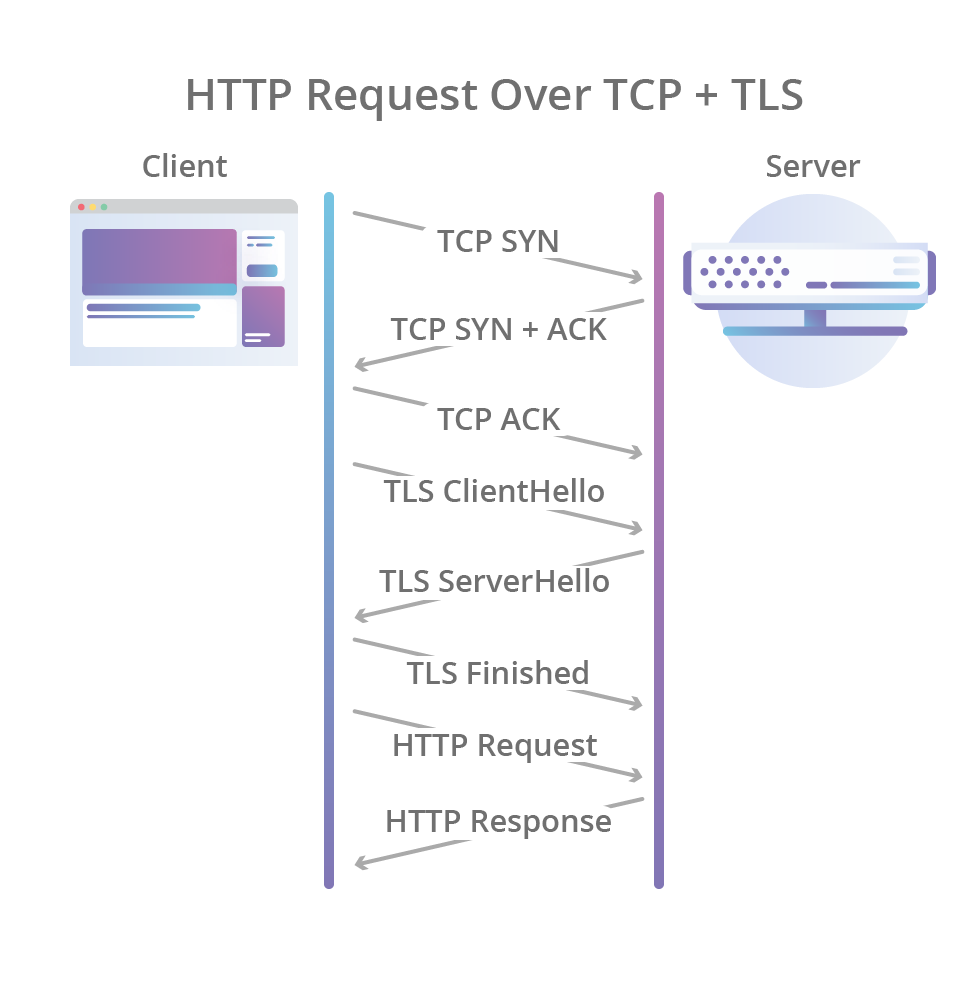
\includegraphics[width=0.45\textwidth]{img/02_stateofart/tcp+tls_handshake.png}}}
        \qquad
        \subfloat[\centering QUIC Handshake]{{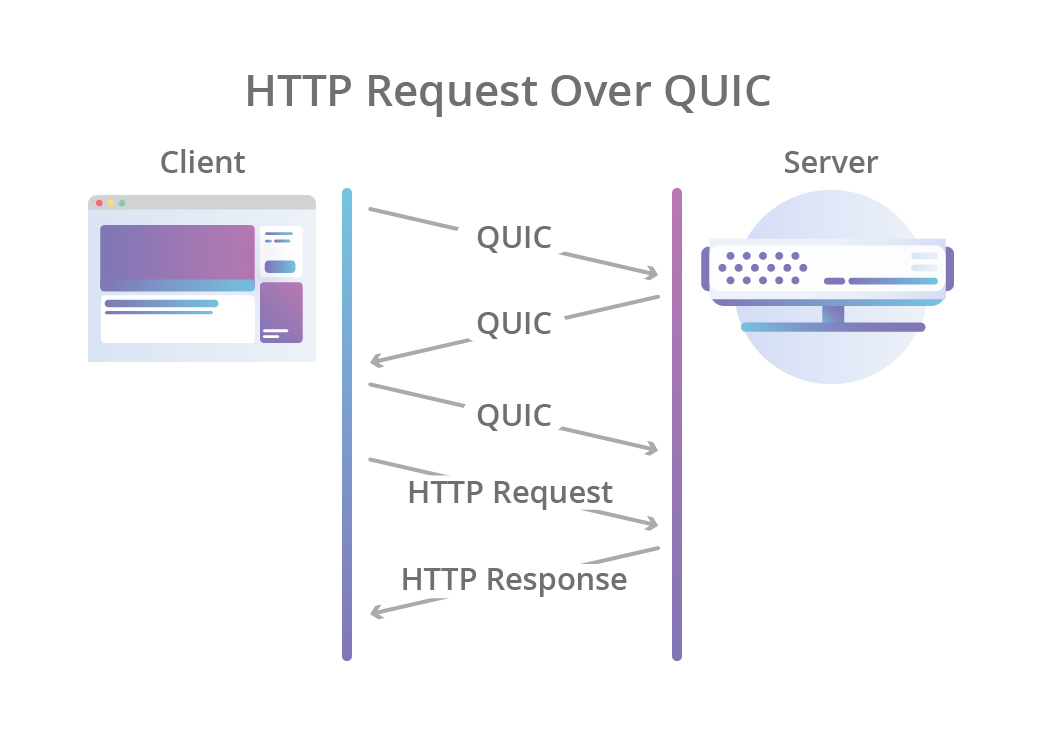
\includegraphics[width=0.45\textwidth]{img/02_stateofart/quic_handshake.png}}}
        \caption{Comparativa establiment connexió entre TCP+TLS i QUIC. Imatge de Cloudflare.}
        \label{fig:comparativa_handshakes}%
    \end{figure}
 
}

\subsubsection{QUIC: Migració}
{
    A QUIC al mateix temps s'introdueix un concepte molt interessant que és el \textbf{Connection ID}. Bàsicament, es tracta d'un tiquet l'identifica la teva connexió. Això comporta grans avantatges com la fàcil migració de connexió que a continuació s'explica, que en el
    mateix port puguin córrer diverses aplicacions, principalment a la banda del client o ajudar a evitar atacs d'amplificació (s'explica
    en detall en el RFC 9000).

    Fins ara, quan s'estableix la connexió, sempre es parlava d'una tupla per identificar a l'altre extrem: una IP i un port. Aquest
    plantejament de baix nivell funciona molt bé per dispositius que no canvien de xarxa o IP. Tanmateix, amb la vinguda dels dispositius
    mòbils i sobretot dels smartphones aquest concepte d'identificar a l'altre extrem amb la IP i el port pot arribar a ser un problema, ja
    que aquest canvien de xarxa mòbil a xarxa wifi bastant sovint. Això no permet reprendre una connexió a on s'havia deixat si s'estaven enviant
    dades havent de tornar a fer el \textit{handshake} un altre cop. Amb QUIC i el plantejament d'identificadors de connexió o
    \textit{Connection ID}s canvia completament.

    A QUIC s'introdueix el concepte de \textbf{0-RTT}; és a dir, que encara que és canvi de xarxa la connexió es pot reprendre a on s'havia deixat
    evitant fer tants de \textit{handshakes} i pràcticament transmetre dades des de la primera resposta si s'ha establert una connexió anteriorment.
    Per aconseguir això, tant el servidor com el client ha de mantenir una sèrie de paràmetres de transport (principalment de TLS) i el mateix
    \textit{Connection ID} tant en la banda del servidor com del client (detalls a la secció 7 de [QUIC-Transport]).
    
}

\subsubsection{QUIC: capçaleres més dinàmiques}
{
    A QUIC hi ha dos tipus principals de paquets en termes de mida i el que duen\footnote{ S'adjunta el següent enllaç on s'expliquen en una mica
    detall tots els tipus: https://gist.github.com/martinthomson/744d04cbcec9be554f2f8e7bae2715b8}.
    Per una banda, están els paquets amb una capçalera llarga o
    \textit{long header} que són utilitzat principalment durant els \textit{handshakes} o altres paquets especials.
    Aquest tipus de paquets inclouen el \textit{SCID} (\textit{Source Connection ID}), el \textit{DCID}
    (\textit{Destination Connection ID}), altres paràmetres de transport, etc. Aquests paquets també poden dur càrrega útil de capes superiors, encara
    que aquest tipus no és el més adequat per connexions llargues.
    
    Per altra banda, hi ha un altre tipus de paquets que tenen una capçalera curta o \textit{short header} que sí que són emprats després que la
    connexió s'ha establert i es transfereixen les dades de manera més extensa. Aquest tipus de paquets només duen el \textit{DCID} i el número de paquet
    pràcticament, ja que són les úniques dues dades fonamentals perquè la connexió pugui funcionar.
    
    Si s'ha d'enviar un tipus de trama especial, normalment s'envia a través dels fluxos o \textit{streams} que es generen durant el \textit{handshake}
    o en fases posteriors. Sol haver-hi un canal destinat a aquest tipus de trames.
}

\subsubsection{QUIC: Multiplexat}
{
    Ja des de HTTP/2 s'ha plantejat el concepte de multiplexat en l'enviament de dades. Per ficar context, només la pàgina inicial de la gran
    majoria de pàgines web que podem visitar a través de cercadors estan fetes a base de molts arxius, ja sigui l'arxiu HTML (.html),
    l'arxiu per decorar (.css), l'arxiu per afegir interactivitat (.js) o fotos i altres (.jpg, .mp3, .ts, etc.). En veure aquesta situació
    ja en el seu moment es va platejar que descarregar paral·lelament aquests arxius podia accelerar en gran manera la velocitat de càrrega i
    descarregar al servidor de feina (sobretot si apliquem també \textit{server push}).
    
    Encara que aquesta idea al final si ha millorat molt les velocitats de càrrega, xoca frontalment amb el concepte d'un únic flux de dades
    que proposa TCP. En el cas que es perdi un paquet d'un flux de dades HTTP/2, llavors tots els fluxos han d'esperar al fet que aquest paquet
    es recuperi fent que la millora velocitat que guanyàvem abans es perdi, ja que s'activa el mecanisme de ARQ de TCP. Aquest fenomen s'anomena
    \textit{Head-of-line blocking}.
    
    Amb HTTP/3 (HTTP sobre QUIC), com a la capa de transport s'utilitza UDP, llavors quan es perd un paquet d'un flux de dades, els altres fluxos
    no es veuen interromputs, ja que no hi ha mecanismes en capes inferiors com ARQ com si li passa a HTTP/2 amb TCP. De fet, es pot pensar en cada
    flux de QUIC com un flux TCP independent que incorpora mecanisme de recuperació i validació de paquets.
}

\subsubsection{QUIC: Control de fluxe a nivell de connexió i de paquets de dades}
{
    Donat que es realitza un multiplexat individual per cada \textit{stream} llavors el control de flux s'ha de fer per cada \textit{stream}
    individualment, encara que també es comptabilitza a escala general (mirar més especificacions en la secció 4 de [QUIC-transport]).
    
    A manera de resum molt ràpid, les dades s'envien en trames STREAM i quan l'aplicació de capa superior no vol enviar més dades temporalment s'utilitza
    STREAM\_DATA\_BLOCKED per mantenir la connexió viva. Els fluxos poden ser unidireccionals, des del client al servidor o viceversa, o bidireccionals.
    Els \textit{streams} poden tenir prioritats i és important respectar els estats d'aquests perquè la connexió funcioni (es recomana llegir l'apartat
    3 de [QUIC-transport] per més detalls).
}

\subsubsection{QUIC: Autenticació i encriptació de la capçalera i càrrega útil}
{
    Finalment, per acabar de contar entre altres coses interessants que afegeix QUIC, ens falta parlar dels seus mecanismes d'autenticació i encriptació tant de
    la capçalera com de la càrrega útil. Fins ara, quan s'envia un paquet via TCP, únicament s'encriptava a la càrrega útil i es deixava a capes superiors (TLS)
    aquesta feina. El fet de poder encriptar la majoria de la capçalera i verificar que el receptor és qui realment diu ser fa que atacs del tipus amplificació siguin
    especialment complicats.
}

\subsection{QUIC Multicast}
{
    Com s'ha pogut veure fins ara, QUIC és un protocol destinat per ser unicast completament ja que inclou principalment mecanismes de control de fluxe o 
    retransmissió del paquet entre d'altres. No obstant, es pot arribar a fer un perfil concret de QUIC pel cas de multicast, ja que encara que no s'aprofiti
    tant sí que és útil per evitar les \textit{middleboxes} com routers o firewalls a no tallar el tràfic multicast.

    La avantatge principal que pot oferir fer un perfil concret de QUIC per multicast és que aquest protocol ja està establert com un estàndard. Un dels majors
    problemes de les xarxes de comunicacions actuals resideix a la hora fer actualització de software als \textit{middleboxes} i a vegades la mala implementació
    de certs estàndards (recordar el cas de TLS 1.1 a 1.2 i TLS 1.2 a 1.3). Llavors, el plantejament de fer un estàndard des de 0 normalment no sol ser una bona 
    idea en general.

    Per altra banda, el ús de QUIC podria permetre dues avantatges més. Per una part, el multiplexat pot ser força interessant sobretot per \textit{streamings} 
    de video, ja que en un \textit{stream} es pot enviar la imatge, en un altre l'audio i en un altre els subtitols per exemple. Per altra part, el disposar 
    d'un rang tan gran de \textit{Connections ID}s, 2048 bits, permet destinar una part d'aquest rang per direccions multicast i altra part per els homònims 
    en unicast per senyalització; no obstant, aquesta última proposta també es pot fer amb Session IDs com amb NGHQ i proposa el esborrany de Multicast over QUIC,
    aprofitant el ús de Connection ID 0 (mirar [QUIC Transport]).
    
    De manera molt breu, alguns aspectes tècnics a tenir en compte sobre aquest perfil és que es recomana tenir un canal alternatiu on es faci el \textit{handshake},
    la retransmissió de paquets perduts i demés. la connexió multicast únicament ha d'enviar paquets unidireccionalment del servidor al client en format \textit{short
    header}. Tots els clients han de tenir el mateix \textit{Connection ID} de destí.

    Actualment nomès hi ha un esborrany de l'IETF escrit per Lucas Pardue, Sam Hurst i Richard Bradbury que es diu HTTP sobre QUIC multicast. No obstant, a partir de 
    març de 2022, també l'enginyer de Akamai Jake Holland està escrivint un esborrany al respecte, encara que en aquest cas, actualment està en una fase inicial.
}

\subsection{Software i llibreries importants}
\subsubsection{VNX: Virtual Network over Linux}
{
    És un software general \textit{open-source} de virtualització dissenyat per construir xarxes de proves virtuals automàticament. Permet la definició i 
    desplegament automàtic de escenaris de xarxa construit amb màquines virtuals de diferents tipus (Linux, Windows, FreeBSD, Olive o routers Dynamips, etc)
    interconnectats seguint una topologia definida per l'usuari, permitint inclús connectar aquesta a xarxes externes.

    Esta desenvolupat pel professor David Fernández de l'Universitat Politècnica de Madrid (UPM).
}

\subsubsection{Wireshark}
{
    Wireshark és un programari lliure i de codi obert amb la funcionalitat d'analitzador de paquets de xarxes de comunicació. Wireshark s'empra per 
    a solucionar problemes en xarxes, desenvolupament i anàlisi de programari i tasques educatives. Originàriament s'anomenava Ethereal i va ser 
    reanomenat Wireshark el maig del 2006 per causes comercials.

    Wireshark és molt similar al programari tcpdump, però amb un una interfície gràfica d'usuari i més opcions de menú per a ordenar i filtrar. Es pot
    emprar per analitzar tot tipus de protocols, des de nivell capa 2 com Ethernet fins a nivells superiors com HTTP.
}

\subsubsection{NGTCP2: QUIC unicast}
{
    És una llibreria escrita en C++ que permet enviar missatges unicast utilitzant el protocol QUIC. Està basada en el RFC 9000 [QUIC Transport] i està
    implementat casi tot l'estàndard. Té una sèrie d'exemples bastant útils encara que complicats d'entendre a primer cop d'ull. Als annexes hi ha un exemple
    d'ús del servidor i el client.
}

\subsubsection{NGHQ: QUIC multicast}
{
    És una llibreria desenvolupada en codi C que permet enviar paquets QUIC sobre multicast. Està basada en el part de l'esborrany 7 d'HTTP sobre Multicast QUIC.
    Una llibreria una mica complicada d'utilitzar pero s'han fet petites modificacions per poder adaptar-la al projecte.
    
    Està escrita per Sam Hurst, Lucas Pardue i Richard Bradbury, enginyers de la \ac{BBC}.  
}

\subsubsection{Mencions importants}
{
    \begin{itemize}
        \item \textbf{ffmpeg}: és una eina que permet modificar, retallar, enviar, etc fluxes de videos principalment.
        \item \textbf{smcroute}: Static Multicast Route és una eina que permet crear rutes estàtiques per enrutar el tràfic multicast.
        \item \textbf{mnc}: versió multicast de la clàssica eina Netcat, encara bastant més limitada.
        \item \textbf{mcsender}: emet una senyal multicast cada segon. Serveix per enviar tràfic multicast i comprovar que funciona l'enrutament.
        \item \textbf{vlc}: Visualitzador de video.
        \item \textbf{lxc}: Linux Containers serveix per crear una màquina virtual pero sense haver de crear el kernel. Més eficient que una màquina \ac{KVM}.
    \end{itemize}
}